% Method sections, shared by the report.  Written as part of
% reports/cpm_rotation_3d_results.tex.

\section{What the two tests are}

Both tests solve the same screened problem on a surface in $\mathbb{R}^3$,
\begin{equation}
  u - \Delta_S u = f ,
  \label{eq:pde}
\end{equation}
with a manufactured solution. Both surfaces are made of two pieces. The
pieces meet along a closed curve. The surface is not smooth along that
curve.

A single closest point extension is not available at such a curve. The
medial axis of the surface comes out of the curve. A stencil that crosses
the medial axis couples the two pieces directly. The closest point map is
not single valued there.

Each test therefore uses one band per piece. We call a piece a
\emph{branch}. Each band is complete except at the rows whose own closest
point falls on the shared curve. Those rows have no footpoint of their
own to read. The \emph{angle rotation glue} supplies them. It turns the
grid node rigidly about the shared curve, then projects the turned node
onto the other branch.

\subsection{Test 1: the flipped cap on an ellipsoid}

The surface is the ellipsoid of revolution about the $z$ axis,
\begin{equation}
  \gamma(\varphi,\vartheta) = \bigl(a\sin\varphi\cos\vartheta,\;
  a\sin\varphi\sin\vartheta,\; c\cos\varphi \bigr),
  \qquad \varphi\in[0,\pi],
\end{equation}
with $a=1$ and $c=0.65$. A plane $z=z_{\mathrm{cut}}$ cuts it. Branch~1
is the bowl below the cut. Branch~2 is the cap above the cut.

The cap is then reflected down across the cut plane,
$(x,y,z)\mapsto(x,y,2z_{\mathrm{cut}}-z)$. The cap becomes a dimple
inside the bowl. The two pieces now meet along the whole cut circle in a
crease. This is the \texttt{flipped} case, and it is the default.

A reflection is an isometry. The flipped surface therefore carries the
same metric as the ellipsoid in the same $(\varphi,\vartheta)$. The
manufactured solution and its Laplace--Beltrami operator are the same
functions of $(\varphi,\vartheta)$ on both branches. The errors of the
two branches are directly comparable, and the jump $[f]$ is zero.

The manufactured solution is
\begin{equation}
  u = \cos\varphi + \tfrac12\cos 2\varphi
      + B\sin^2\!\varphi\,\cos 2\vartheta , \qquad B = 0.4 ,
\end{equation}
which is a polynomial in $z$ plus $B(x^2-y^2)/a^2$. It is therefore
smooth at both poles, where the $(\varphi,\vartheta)$ chart is not.
$\Delta_S u$ is analytic.

The script runs four cut heights, written through
$\sin t_c = (z_{\mathrm{cut}} - z_{\mathrm{cen}})/c$:
\begin{equation}
  s_0 = \sin t_c \in \{0.6,\; 0.7,\; 0.8,\; 0.9\} .
\end{equation}
The crease angle and the curvature mismatch grow together as the cut
slides from the pole towards the equator. The list is therefore a list of
curvature mismatches.

\subsection{Test 2: the half-twisted rectangular tube}

The surface is a rectangular tube whose cross-section turns by half a
turn around the centreline circle,
\begin{equation}
  F(\theta,p) = (R+u)\,(\cos\theta,\sin\theta,0) + v\,(0,0,1),
  \qquad
  \begin{aligned}
    u &= p_1\cos\tfrac\theta2 - p_2\sin\tfrac\theta2,\\
    v &= p_1\sin\tfrac\theta2 + p_2\cos\tfrac\theta2,
  \end{aligned}
\end{equation}
with $R=1$, $a=0.45$ and $b=0.20$. The angle $\theta$ is $4\pi$ periodic.
Branch~A (wide) is $p=(s,b)$ with $s\in[-a,a]$. Branch~B (narrow) is
$p=(a,s)$ with $s\in[-b,b]$. Each strip covers its face pair once over
$\theta\in[0,4\pi)$.

The two strips meet along \emph{two} closed curves:
\begin{align}
  \text{upper:}&\quad \text{A at } (\theta,+a)
    \;=\; \text{B at } (\theta,+b), \\
  \text{lower:}&\quad \text{A at } (\theta,-a)
    \;=\; \text{B at } (\theta+2\pi,-b) \pmod{4\pi} .
\end{align}
The shift by $2\pi$ on the lower curve is the half twist. The complete
surface is a closed orientable torus. Figure~\ref{fig:tubegeom} shows it.

The metric of a strip is $E=|F_s|^2=1$, $H=F_s\cdot F_\theta$ (equal to
$-b/2$ on A and $+a/2$ on B), and $G=|F_\theta|^2$. The two faces are not
exactly perpendicular, because of the twist. The glue angle therefore
varies along each curve. This is the main difference from the ellipsoid,
where one angle serves the whole cut circle.

The manufactured solution is, on each strip, the cubic Hermite
interpolant in $s$ between edge traces and edge slopes. The traces and
slopes vary smoothly in $\theta$. Both strips use the same trace on each
curve. The slopes are chosen so that the two outgoing conormal fluxes sum
to zero on both curves. The traces therefore agree and the fluxes
balance, which is what the transmission conditions ask for. The forcing
$f=u-\Delta_S u$ is analytic to rounding.

\section{How we build the grid}

Both tests use \emph{one} Cartesian grid and \emph{two} bands on it. The
shared grid is what makes the cross-branch block of the operator
assemblable. With one grid per branch there is no common column index
space, and an extra grid-to-grid transfer would pollute the glue error we
want to measure.

\subsection{Bandwidth}

Both tests take the bandwidth from the Ruuth--Merriman formula
\cite{RuuthMerriman2008},
\begin{equation}
  \mathrm{bw} = 1.0002\,
  \sqrt{(d-1)\Bigl(\tfrac{p+1}{2}\Bigr)^{\!2}
        + \Bigl(\tfrac{q}{2}+\tfrac{p+1}{2}\Bigr)^{\!2}} ,
  \label{eq:bw}
\end{equation}
with $d=3$, interpolation degree $p=3$ and Laplacian order $q=2$. This
gives $\mathrm{bw}\approx 4.12$. The factor $1.0002$ is a safety factor.
The two tangential directions of a surface each contribute one
interpolation half-stencil. The normal direction contributes one
interpolation half-stencil plus one Laplacian half-stencil. That is what
the composition $EL$ reads.

\subsection{The box and the grid offsets}

The box is the bounding box of the two pieces \emph{as they are
embedded}, plus a pad of a few cells. For the flipped ellipsoid the box
is much shorter in $z$ than the ellipsoid's own box, because the cap is
folded inside the bowl. For the tube the box comes from the centreline
radius $R$ plus the cross-section radius $\rho=\sqrt{a^2+b^2}$.

Each axis is then shifted by an odd fraction of the grid spacing:
\begin{center}
\begin{tabular}{lll}
  \toprule
  Test & shift of $(x,y,z)$ in units of $h$ \\
  \midrule
  flipped ellipsoid & $(-0.317,\; -0.211,\; -0.133)$ \\
  half-twisted tube & $(+0.317,\; +0.211,\; +0.173)$ \\
  \bottomrule
\end{tabular}
\end{center}
The shifts matter. A grid that is symmetric about the cut plane gives the
two branches mirror-image tangent estimates. The errors of those
estimates then cancel in the glue rotation, and the estimator looks
better than it is. The shifts also keep the junction curve off the grid
nodes.

\subsection{Finding the nodes near the surface}

A full \texttt{meshgrid} over the box cannot be built at the finest grid
spacing, and the banding would discard all but a shell of it. Each test
therefore prefilters first.

\paragraph{Ellipsoid.} The script walks each piece in the polar angle
$\varphi$, and at each $\varphi$ around the parallel with a count set by
that parallel's own circumference. The poles are therefore not
oversampled. Samples are no more than about $h/2$ apart. Each sample is
snapped to the nearest grid node. The seed set is then grown by
$\mathrm{rad}=\lceil \mathrm{bw}\rceil+2$ cells, one axis at a time, with
unique linear indices taken after each axis. The working set stays the
size of the band instead of $(2\,\mathrm{rad}+1)^3$ times it.

\paragraph{Tube.} Every strip point lies within $\rho$ of the centreline
circle. A node within $\mathrm{bw}\,h$ of either strip is therefore
within $\rho+\mathrm{bw}\,h$ of that circle. The prefilter keeps the
nodes with
\begin{equation}
  \bigl(\sqrt{x^2+y^2}-R\bigr)^2 + z^2
  \;\le\; (\rho + \mathrm{bw}\,h)^2 .
\end{equation}
This is the \emph{conservative initial band}. Everything the operator
needs must lie inside it, or the run stops with an error.

\subsection{From candidates to bands}

Each branch then runs its \emph{own} closest point function over the
candidate nodes. The ellipsoid uses \texttt{cpEllipseArc} in the meridian
half plane, spun back out along the azimuth of the query; a reflected
piece is handled by reflecting the query, solving, and reflecting the
answer. The tube uses \texttt{cpHalfTwistedRectTube}, which clamps $s$
exactly for fixed $\theta$ and then refines $\theta$ by safeguarded
Newton iteration from 256 periodic samples.

A node is kept when $|\mathrm{dist}| \le \mathrm{bw}\,h$. Near the
junction curve a node lies in \emph{both} bands. It then carries
\emph{two} independent unknowns, one per branch field. The bands overlap
in space; the unknowns never overlap.

The two tests then differ in how the band is closed.

\paragraph{Ellipsoid: one band per branch.} The vGMM operator applies $L$
to the band values and extends the result. $E$ and $L$ are therefore both
square on the same node set, and no restriction operator is needed. The
script marks the rows of $L$ whose whole stencil landed in the band
(\texttt{lfull}). A row at the outer edge loses part of its stencil. That
is harmless while nothing reads the row, and the script checks that: in
$EL$ a row of $L$ is read only when $E$ has a nonzero in that column.

\paragraph{Tube: inner band, outer band, and a closure sweep.} The inner
band of a branch must hold every interpolation stencil used on it. Three
sets of stencils must fit:
\begin{enumerate}
  \item the stencils of the closest points of its own initial band;
  \item the stencils of every surface error sample and every
        corner-curve trace sample;
  \item the stencils of the target closest points of the rows routed
        \emph{into} it, by \emph{either} rotation.
\end{enumerate}
The outer band is the inner band plus its 7-point Laplacian neighbours.
Enlarging an inner band enlarges the outer band. A larger outer band can
create new routed rows, and those rows need new support. Banding and
routing are therefore iterated until nothing new appears. The sweep count
is reported. Both rotation methods share one set of bands and one set of
routed rows, so only the angle differs between them.

\subsection{The grid spacings}

The flipped ellipsoid uses $h_k = 0.065\times 0.82^{\,k}$. A band node
has a unique closest point on its branch only while $\mathrm{bw}\,h$
stays below the smallest radius of curvature, which on an oblate
ellipsoid is $c^2/a$ at the equator. The script keeps only the $h$ that
satisfy $\mathrm{bw}\,h < 0.65\min(c^2/a,\, a^2/c)$.

Many grid spacings are needed, and the reason is specific to this
surface. The surface error of the flipped solve is \emph{not} a smooth
function of $h$. Its size is set by the net signed junction residual
summed around the cut circle. That sum is a near cancellation: each
branch contributes a systematic total of one sign, the other branch the
opposite sign. What survives depends on where the cut circle falls
between grid planes. Neighbouring $h$ can differ by a factor of several,
and a level-to-level rate is meaningless. Only the least-squares slope
through many levels is a rate. In the plane the same cancellation exists,
but the junction is two points instead of a circle, the sums run over
$O(1)$ rows instead of $O(1/h)$ rows, and the noise never surfaces.

The tube uses an explicit list of $h$, and rates use the actual ratios.

\section{How we find and apply the rotation}

% Schematic of the angle rotation glue, in the plane normal to the
% junction curve.  Included by cpm_rotation_3d_results.tex.
%
% Convention: eta_t is the target branch's OUTWARD conormal, so the
% target branch itself lies along -eta_t.  The glue carries eta_s onto
% -eta_t, which is why the rotated node lands beside the target branch.
\begin{figure}[htbp]
\centering
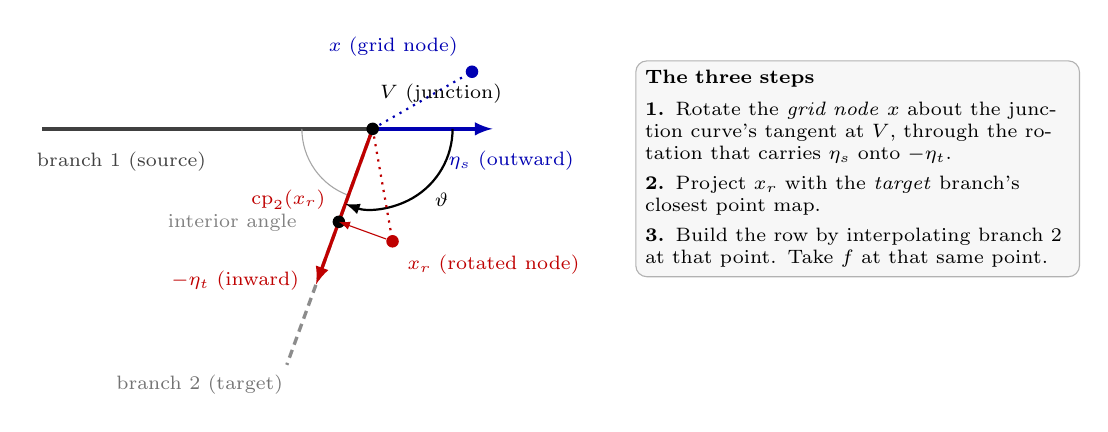
\begin{tikzpicture}[scale=1.45,>=latex,
    srcface/.style={very thick, black!75},
    tgtface/.style={very thick, black!45, densely dashed},
    node1/.style={circle, fill=blue!70!black, inner sep=1.6pt},
    node2/.style={circle, fill=red!75!black, inner sep=1.6pt},
    cp/.style={circle, fill=black, inner sep=1.6pt},
    lbl/.style={font=\scriptsize}]

  \coordinate (V) at (0,0);

  % ---- branch 1: the source face, along 180 degrees ----
  \draw[srcface] (V) -- (-2.90,0);
  \node[lbl, black!75, anchor=north] at (-2.20,-0.12)
      {branch 1 (source)};

  % ---- branch 2: the target face, along 250 degrees ----
  \draw[tgtface] (V) -- (-0.752,-2.067);
  \node[lbl, black!55, anchor=north east] at (-0.70,-2.07)
      {branch 2 (target)};

  % ---- the interior angle at the junction ----
  \draw[black!35] (-0.62,0) arc[start angle=180, end angle=250,
      radius=0.62];
  \node[lbl, black!50, anchor=north east] at (-0.58,-0.66)
      {interior angle};

  % ---- outward conormal of the source ----
  \draw[->, very thick, blue!70!black] (V) -- (1.05,0);
  \node[lbl, blue!70!black, anchor=north west] at (0.58,-0.11)
      {$\eta_s$ (outward)};

  % ---- inward direction of the target, along branch 2 ----
  \draw[->, very thick, red!75!black] (V) -- (-0.496,-1.363);
  \node[lbl, red!75!black, anchor=east] at (-0.56,-1.33)
      {$-\eta_t$ (inward)};

  % ---- the glue rotation ----
  \draw[->, thick, black] (0.70,0) arc[start angle=0,
      end angle=-110, radius=0.70];
  \node[lbl, anchor=west] at (0.46,-0.62) {$\vartheta$};

  % ---- the grid node, and its rotated image ----
  \node[node1] (X) at (0.87,0.50) {};
  \node[lbl, blue!70!black, anchor=south east] at (0.83,0.55)
      {$x$ (grid node)};
  \draw[blue!70!black, dotted, thick] (V) -- (X);

  \node[node2] (XR) at (0.174,-0.985) {};
  \node[lbl, red!75!black, anchor=north west] at (0.22,-1.02)
      {$x_r$ (rotated node)};
  \draw[red!75!black, dotted, thick] (V) -- (XR);

  % ---- the closest point of the rotated node on branch 2 ----
  \coordinate (CPT) at (-0.296,-0.814);
  \node[cp] at (CPT) {};
  \draw[->, red!75!black, thin] (XR) -- (CPT);
  \node[lbl, red!75!black, anchor=south east] at (-0.33,-0.79)
      {$\mathrm{cp}_2(x_r)$};

  \node[cp] at (V) {};
  \node[lbl, anchor=south west] at (-0.02,0.14) {$V$ (junction)};

  % ---- annotation box, clear of the drawing ----
  \node[draw=black!30, fill=black!3, rounded corners, align=left,
        lbl, text width=5.4cm, anchor=north west] at (2.30,0.60)
      {\textbf{The three steps}\\[1.2mm]
       \textbf{1.} Rotate the \emph{grid node} $x$ about the junction
          curve's tangent at $V$, through the rotation that carries
          $\eta_s$ onto $-\eta_t$.\\[1mm]
       \textbf{2.} Project $x_r$ with the \emph{target} branch's
          closest point map.\\[1mm]
       \textbf{3.} Build the row by interpolating branch 2 at that
          point. Take $f$ at that same point.};

\end{tikzpicture}
\caption{The angle rotation glue, drawn in the plane normal to the
  junction curve. Here $\eta_t$ is the target branch's \emph{outward}
  conormal, so branch 2 itself lies along $-\eta_t$. The rotation carries
  the source branch's outward direction $\eta_s$ onto $-\eta_t$. Leaving
  one branch means entering the other, so outward-onto-inward is the
  pairing a rigid continuation needs. The object that is rotated is the
  grid node $x$, not its closest point. This carries both the overhang
  past the junction and the normal offset across intact. On the ellipsoid
  this plane is a meridian half plane, and one angle serves the whole cut
  circle. On the tube the plane is the normal plane of a corner curve,
  and the angle varies along the curve, because the twist stops the two
  faces from being perpendicular.}
\label{fig:glue}
\end{figure}



\subsection{Which rows are rotated}

A row is rotated when its own closest point lies on the junction curve.

On the ellipsoid, \texttt{cpEllipseArc} returns the clamped end of the
meridian arc exactly. The test is therefore done on the meridian
coordinates $(\rho,z)$ of the closest point, with the reflection undone
first, to a tolerance of $10^4\,\varepsilon$. The poles are the other
ends of the two meridian arcs. They are not boundaries, because the
surface of revolution closes up there, and they are correctly not
matched.

On the tube, the closest point function returns a flag
$\mathrm{bdy}=\pm1$ when the closest point lies on the edge $s=\mp W$.
Every outer row with $\mathrm{bdy}\neq0$ is routed.

\subsection{The rotation axis}

The axis is the tangent to the junction curve at the row's own closest
point.

On the ellipsoid that tangent is the azimuthal direction
$e_\vartheta$. Two facts make this the honest lift of the planar
construction. First, the closest point $V$ of the node lies on a
\emph{circle}, so the offset of the node from $V$ has no $e_\vartheta$
component; the node lies in $V$'s own meridian half plane, and a rotation
about $e_\vartheta$ keeps it there. Second, the surface is one of
revolution, so the closest point of the rotated node on the other branch
lies in the same half plane. The whole construction is the planar one,
applied meridian by meridian, and the angle is the planar angle in the
$(\rho,z)$ coordinates of that half plane.

On the tube the axis is $\tau = F_\theta/|F_\theta|$ at the edge closest
point. Both strips share it. Both methods use the analytic $\tau$.

\subsection{The angle}

The glue carries the \emph{outward} direction of the source branch onto
the \emph{inward} direction of the target branch. Leaving the source
branch at the junction means entering the target branch, so
outward-onto-inward is the pairing a rigid continuation needs. On a
smooth join the two directions are opposite and the rotation is the
identity.

On the ellipsoid the two directions are the outward unit tangents of the
two meridian arcs at the cut. Reflecting branch~2 negates the $z$
component of its tangent, and that is what opens the crease. At
$s_0=0.6$, for example, the exact glue angle is $1.4282$~rad
($81.8^\circ$).

On the tube the two directions are the outward conormals,
\begin{equation}
  \eta_s = \operatorname{sign}(s)\,
  \mathrm{unit}\bigl(F_s - (F_s\!\cdot\!\tau)\tau\bigr),
\end{equation}
on the source strip, and $\eta_t$ likewise on the target strip at the
glued parameters. The glue carries $\eta_s$ onto $-\eta_t$. Because of
the twist this angle varies along the curve, so it is computed per row.

\subsection{The construction: Rodrigues, not \texttt{atan2}}

Nothing in this code stores a glue angle. The rotation is stored as a
$(\cos,\sin)$ pair, and the pair comes straight out of the two
directions. Rodrigues' formula about a unit axis $k$ is
\begin{equation}
  R = I + \sin\vartheta\,K + (1-\cos\vartheta)\,K^2 ,
  \qquad K = \mathrm{skew}(k) .
\end{equation}
In the plane the axis is $e_z$, $K^2=-I$, and the formula collapses to
$R = \cos\vartheta\,I + \sin\vartheta\,K = \begin{bmatrix} c & -s\\ s &
c\end{bmatrix}$ with
\begin{equation}
  c = u\cdot w , \qquad
  s = (u\times w)\cdot e_z = u_1w_2 - u_2w_1 ,
\end{equation}
followed by one division by $\mathrm{hypot}(c,s)$. In three dimensions
the same two quantities are $c = u\cdot w$ and
$s = \tau\cdot(u\times w)$. No angle is formed and no transcendental
function is evaluated.

The angle-first alternative reaches the same matrix through six library
transcendental calls, and $\cos$ and $\sin$ immediately undo what
\texttt{atan2} just did. Four consequences follow, and the planar
companion experiment measures all of them:
\begin{itemize}
  \item \textbf{Accuracy.} Against a rotation known to full precision,
        $\|R-R_{\mathrm{exact}}\|$ comes out two to seven times larger
        for the angle-first path at every angle sampled over a full turn.
        The worst case over that sweep is $1.2\times10^{-15}$ against
        $2.8\times10^{-16}$. Both are a few units in the last place, so
        this is a reason to prefer the construction, not a defect being
        repaired.
  \item \textbf{No branch cut.} A difference of two \texttt{atan2} values
        lands in $(-2\pi,2\pi]$ and must be wrapped back. The stored
        number is then discontinuous at $\pm\pi$, although the rotation
        it stands for is not. A $(\cos,\sin)$ pair has no such seam.
  \item \textbf{Exact inverses.} Swapping the two directions gives the
        other branch's glue at the same junction point. Under Rodrigues
        the cosine comes out bit for bit the same and the sine bit for
        bit negated, so the two branches' rotations are \emph{exact}
        transposes. The angle-first path satisfies that only to within
        rounding.
  \item \textbf{Reproducibility.} IEEE~754 pins down multiply, add,
        divide and \texttt{hypot}. It says nothing about \texttt{atan2},
        \texttt{sin} or \texttt{cos}. Dot products, cross products and
        \texttt{hypot} cannot differ between platforms; the angle-first
        matrix can.
\end{itemize}

\subsection{The estimated rotations}

The exact rotation uses analytic directions. It is the reference. Each
test also runs rotations built only from closest point differences,
because a real application has no analytic frame.

Write $\mathrm{cp}$ for the closest point of the node $x$ on its own
branch, and reflect the node through it:
\begin{align}
  \overline{\mathrm{cp}} &= \mathrm{cp}(2\,\mathrm{cp}-x), &
  \overline{\overline{\mathrm{cp}}} &= \mathrm{cp}(3\,\mathrm{cp}-2x) .
\end{align}
The two estimators are
\begin{align}
  d_k   &= \mathrm{cp} - \overline{\mathrm{cp}}
           &&\text{(first order)}, \\
  d_{k2} &= 1.5\,\mathrm{cp} - 2\,\overline{\mathrm{cp}}
            + 0.5\,\overline{\overline{\mathrm{cp}}}
           &&\text{(second order)} .
\end{align}
A plain difference of closest points returns nothing at these rows,
because the closest point \emph{is} the junction point. That is why the
node is reflected first.

\paragraph{Ellipsoid.} Each difference is resolved in its own node's
meridian frame $(e_\rho,e_z)$ \emph{before} averaging. By rotational
symmetry that is the frame the glue angle is measured in. Averaging the
raw vectors instead would cancel them around the circle. The
$e_\vartheta$ component is discarded; it is zero for the exact tangent
and only noise here. The script runs three variants per cut: $d_k$,
$d_{k2}$, and the exact rotation.

\paragraph{Tube.} Both conormals are estimated by $d_{k2}$, projected off
the exact $\tau$ and normalized. The source estimate reflects the
original routed grid node, $v = c-x$. A row is re-sampled with a
deterministic outward probe $x' = c + h\,\eta_s$ when any of these holds:
$|v|$ is tiny; the projected difference is short relative to $|v|$
($\alpha = |d_\perp|/|v| < 0.25$); a reflected closest point is itself on
an edge; the sample jumps to the opposite sheet; or the estimate points
inward. The target estimate always uses the outward probe
$c_t + h\,\eta_t$. An unusable probe raises an error; there is no
fallback to the exact conormal.

This makes the tube's $d_{k2}$ \emph{not} a fully geometry-free
estimator, and the script says so. The exact $\tau$ supplies the axis and
the projection plane. The exact conormals place the probes and check the
outward orientation. Both directions that set the angle are still closest
point differences.

\subsection{Applying the rotation}

We rotate the \emph{grid node}, never its closest point. That is what
makes the map a rigid continuation: both the tangential overhang past the
junction and the normal offset are carried across intact. Rotating the
closest point instead would only reparametrize the junction curve, and it
would lose the normal coordinate.

On the ellipsoid, the offset $x-V$ is resolved in the node's own meridian
frame into $(d_\rho, d_\vartheta, d_z)$. The planar rotation is applied
to $(d_\rho, d_z)$. The component $d_\vartheta$ is zero up to rounding,
and it is carried through anyway, so the formula does not quietly depend
on it vanishing. The result is mapped back to Cartesian coordinates.

On the tube, Rodrigues' formula is applied directly,
\begin{equation}
  x_r = c + (x-c)\cos\vartheta + \bigl(\tau\times(x-c)\bigr)\sin\vartheta
        + \tau\,\bigl(\tau\cdot(x-c)\bigr)(1-\cos\vartheta) ,
\end{equation}
again from the $(\cos,\sin)$ pair and not from an angle.

The rotated node is then projected with the \emph{target} branch's
closest point function. The interpolation stencil is built there.

\subsection{Measuring the rotation error}

The error of an estimated rotation is reported through the \emph{relative}
rotation $R_{\mathrm{exact}}^{\!\top} R$, whose angle lands in
$(-\pi,\pi]$ by construction:
\begin{equation}
  c_{\mathrm{rel}} = c\,c_{\mathrm{ref}} + s\,s_{\mathrm{ref}},
  \qquad
  s_{\mathrm{rel}} = s\,c_{\mathrm{ref}} - c\,s_{\mathrm{ref}} .
\end{equation}
There is nothing to re-wrap. The obvious alternative, a wrapped
difference of two angles, loses digits exactly where the comparison
matters, which is when both angles sit near $\pm\pi$.

\section{How we form the operator}

\subsection{Test 1: the vGMM operator}

The ellipsoid test uses the embedded method-of-lines operator of von
Glehn, M\"arz and Macdonald \cite{vGMM2013},
\begin{equation}
  M = EL - \gamma\,(I-E), \qquad \gamma = \frac{2d}{h^2},
  \label{eq:vgmm}
\end{equation}
and solves $(I-M)\,u = f$. Here $E$ is the degree-3 interpolation at the
closest points, square on the band, and $L$ is the second-order 7-point
Laplacian on the same band.

The glue needs no further handling, and that is the attraction of this
operator. $L$ is block diagonal, so
\begin{equation}
  (EL)_{k,o} = E_{k,o}\,L_o
\end{equation}
extends the \emph{other} branch's $Lu$ across the cut. The stabilization
row $u_i - (Eu)_i$ at a rotated node of branch $k$ is exactly the
statement that branch $k$'s value there agrees with branch $o$'s
interpolant at the rotated point. In assembly, a routed row's entry in
the diagonal block is zeroed, and its weights go into the off-diagonal
block.

$M$ is never assembled. In three dimensions $EL$ has some hundreds of
entries per row; $E$ and $L$ separately have 64 and 7. The operator is
applied as
\begin{equation}
  (I-M)\,v = (1+\gamma)\,v - E\bigl(Lv + \gamma v\bigr) ,
\end{equation}
under restarted GMRES with a Jacobi preconditioner built from
$\operatorname{diag}(EL)_i = \sum_j E_{ij}L_{ji}$. The tolerance is
$10^{-10}$, the restart is 40, and the cap is 400 restart cycles.

\paragraph{The forcing at a junction row.} A rotated row's unknown does
not stand for $u$ at that row's own closest point. That point is on the
cut circle. It stands for $u$ at the rotated target on the other branch,
which is up to $\mathrm{bw}\,h$ of arclength away. Its forcing is
therefore $f$ at the \emph{rotated target}.

This is the one place where the three-dimensional script deliberately
differs from its planar companion, and the reason is a counting argument.
Using $f$ at the row's own clamped closest point leaves a residual
$f(\text{target}) - f(V) = O(h)$ on every one of those rows. With $O(1)$
such rows in the plane that is invisible. With $O(1/h)$ of them around a
circle it is not.

That choice needs a caveat, because it is the convention the surface
analysis singles out as the dangerous one. Evaluating the forcing on the
opposite side without correcting a trace jump can leave the forcing
residual at $O(1)$ instead of $O(h)$, and that would promote its
contribution from $O(h^2)$ to $O(h)$. It is safe here only because
$[f]=0$: $u$ and $f$ are the same functions of $(\varphi,\vartheta)$ on
both branches, so the two one-sided traces agree and there is no jump to
correct. A forcing written per branch rather than per
$(\varphi,\vartheta)$ would break that, and would then need $f$ at the
source-side edge point or an explicit trace correction.

\paragraph{The baseline.} The same vGMM operator is also run on
\emph{one} band over the union of the two pieces. On the unflipped
surface that is the plain ellipsoid, and it measures the uncut rate. On
the flipped surface it is the closest point method applied to the crease
\emph{as if the crease were not there}. That is the other number worth
having.

\subsection{Test 2: the stabilized (diagonally split) ICPM operator}

The tube test uses the diagonally split operator. Let $L$ be the 7-point
Laplacian from the inner band rows to the outer band columns, and $R$ the
restriction from outer to inner. Split $L$ by its own diagonal,
\begin{equation}
  L_{\mathrm{diag}} = \textstyle\sum_j (R\odot L)_{ij}, \qquad
  L_{\mathrm{off}} = L - R\odot L ,
\end{equation}
and form
\begin{equation}
  M = \operatorname{diag}(L_{\mathrm{diag}})
      + L_{\mathrm{off}}\,E ,
  \label{eq:icpm}
\end{equation}
then solve $(I-M)\,u = R\,f_{\mathrm{out}}$.

The extension $E$ is split in two. $E_{\mathrm{self}}$ holds the
non-routed rows; the routed rows of the diagonal block are zeroed.
$E_{\mathrm{cross}}$ holds the routed rows, which interpolate the target
branch at the closest point of the rotated node.

The right-hand side is the source branch's $f$ at the outer rows. On a
routed row it is overwritten by the \emph{target} branch's $f$ at the
target closest point, for the same reason as above.

The solve is a sparse direct solve while the unknown count stays at or
below $25\,000$, and matrix-free restarted GMRES otherwise, with the
$(I-L_{\mathrm{diag}})$ diagonal preconditioner, tolerance $10^{-10}$,
restart 80 and 200 outer cycles. A GMRES failure is an error, not a
warning. The residual of the returned solution is recomputed and stored.

\subsection{What the scripts refuse to do}

Both tests are written so that a silently thinned band is impossible.
Each of the following raises an error rather than a warning:
\begin{itemize}
  \item an interpolation stencil of a closest point leaves the band;
  \item a cross-junction stencil leaves the \emph{other} band;
  \item a cross-junction stencil reads a row whose Laplacian stencil is
        incomplete;
  \item a row sum of the extension differs from one by more than
        $10^{-10}$;
  \item the band or routing closure does not converge in the allowed
        sweeps;
  \item the linear solve does not reach its residual target;
  \item a $d_{k2}$ probe is still unusable after the fallback probe.
\end{itemize}
The row sums and the linear residual are reported per level, so the
tables below can be read against them.

\section{How we measure the error}

The reported quantity is the surface $L_\infty$ error of the
\emph{interpolant}, not of the band values.

On the ellipsoid, each branch is sampled at the midpoints of a uniform
partition of its polar-angle interval, and around each parallel with a
count set by that parallel's own circumference. No sample falls exactly
on the cut circle or at a pole. A sample whose interpolation stencil is
not entirely inside the band is dropped and counted. The script also
records \emph{where} the worst point sits, as an arclength from the cut
circle in multiples of $h$. That is the test of whether the crease is
what hurts the solve.

On the tube, each strip is sampled on a uniform $(\theta,s)$ grid with
about two samples per $h$ in each direction, and \emph{both} edge curves
are included. The script also reports the trace discrepancy of the two
branches on each corner curve.

The ellipsoid test reports four further cross-branch measures at the
nodes the two bands have in common:
\begin{center}
\begin{tabular}{ll}
  \toprule
  measure & definition \\
  \midrule
  \texttt{gap}    & $\max|e_A - e_B|$ at the shared rotated nodes \\
  \texttt{vtx}    & $\max|u_A - u_B|$ on the cut circle \\
  \texttt{branch} & $\max(|e_A|, |e_B|)$ at the same nodes \\
  \texttt{allgap} & $\max|e_A - e_B|$ over the whole overlap \\
  \bottomrule
\end{tabular}
\end{center}
Each branch is compared against the value its \emph{own} unknown stands
for. At a crease the raw difference of the two unknowns is $O(h)$
whatever the scheme does, because the two unknowns stand for $u$ at
different points. What has to be compared is each branch's own error.
